\documentclass[tikz]{standalone}
\usepackage{tikz}
\usetikzlibrary{arrows.meta,positioning,shapes.geometric,shapes.misc,fit,backgrounds,calc,decorations.pathreplacing}

\definecolor{cEmpirical}{HTML}{2B7A78}
\definecolor{cConjectured}{HTML}{C07C38}
\definecolor{cSpeculative}{HTML}{A04050}
\definecolor{cLimit}{HTML}{6B5CA5}

\begin{document}
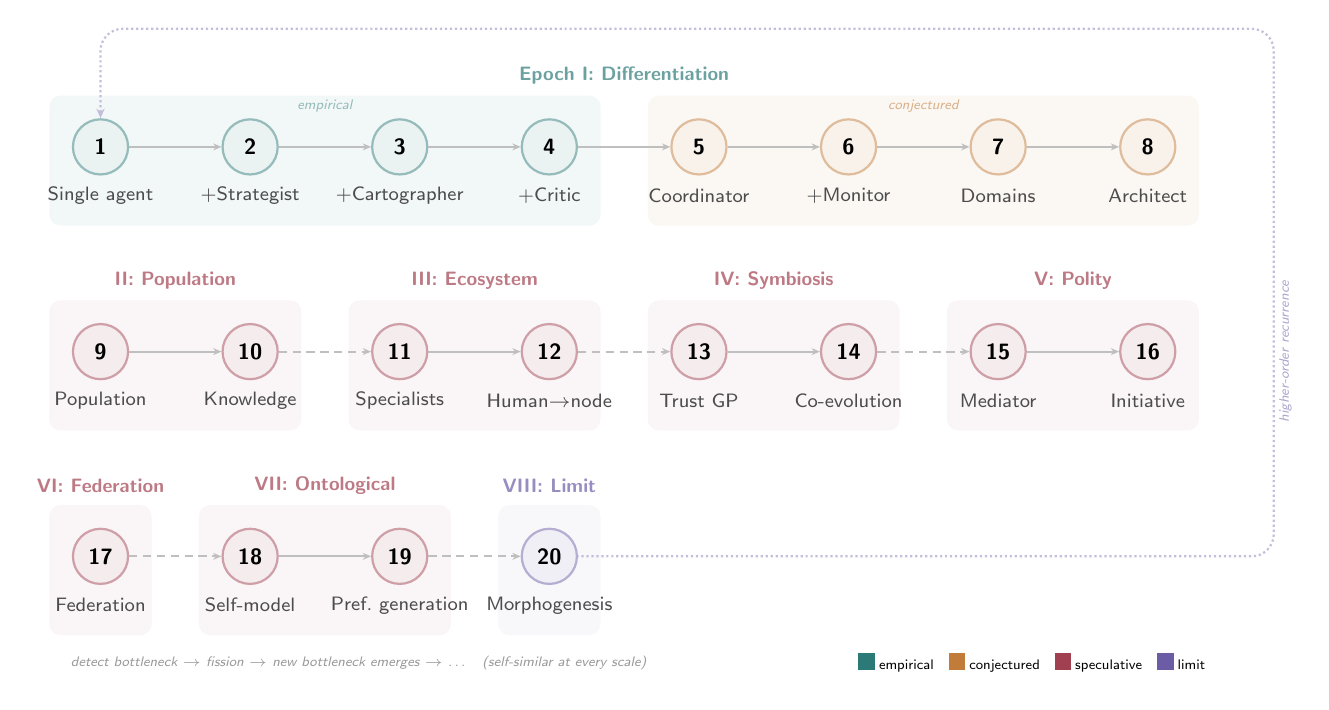
\begin{tikzpicture}[
    ph/.style={circle, draw=#1!50, fill=#1!10, thick,
        minimum size=0.7cm, font=\footnotesize\sffamily\bfseries,
        inner sep=0pt},
    lbl/.style={font=\scriptsize\sffamily, text=black!70, align=center},
    elbl/.style={font=\scriptsize\sffamily\bfseries, text=black!55},
    arr/.style={-{Stealth[length=3pt, width=2.5pt]}, thick, black!25},
    rowarr/.style={-{Stealth[length=3pt, width=2.5pt]}, black!20, thick},
]

\def\xs{1.9}   % x spacing between phases
\def\ys{2.6}   % y spacing between rows

% ============================================================
% ROW 1: Epoch I — Differentiation (Phases 1–8)
% ============================================================

\def\rone{0}

% Epoch backgrounds
\begin{scope}[on background layer]
    \fill[cEmpirical!6, rounded corners=4pt]
        (-0.65, \rone+0.65) rectangle (3*\xs+0.65, \rone-1.0);
    \fill[cConjectured!6, rounded corners=4pt]
        (4*\xs-0.65, \rone+0.65) rectangle (7*\xs+0.65, \rone-1.0);
\end{scope}

% Phase nodes
\node[ph=cEmpirical]   (p1) at (0, \rone) {1};
\node[ph=cEmpirical]   (p2) at (\xs, \rone) {2};
\node[ph=cEmpirical]   (p3) at (2*\xs, \rone) {3};
\node[ph=cEmpirical]   (p4) at (3*\xs, \rone) {4};
\node[ph=cConjectured] (p5) at (4*\xs, \rone) {5};
\node[ph=cConjectured] (p6) at (5*\xs, \rone) {6};
\node[ph=cConjectured] (p7) at (6*\xs, \rone) {7};
\node[ph=cConjectured] (p8) at (7*\xs, \rone) {8};

\foreach \i/\j in {1/2,2/3,3/4,4/5,5/6,6/7,7/8} { \draw[arr] (p\i) -- (p\j); }

% Labels below nodes
\node[lbl] at (0, \rone-0.62)      {Single agent};
\node[lbl] at (\xs, \rone-0.62)    {+Strategist};
\node[lbl] at (2*\xs, \rone-0.62)  {+Cartographer};
\node[lbl] at (3*\xs, \rone-0.62)  {+Critic};
\node[lbl] at (4*\xs, \rone-0.62)  {Coordinator};
\node[lbl] at (5*\xs, \rone-0.62)  {+Monitor};
\node[lbl] at (6*\xs, \rone-0.62)  {Domains};
\node[lbl] at (7*\xs, \rone-0.62)  {Architect};

% Epoch title centered across both halves
\node[elbl, text=cEmpirical!70] at (3.5*\xs, \rone+0.9)
    {Epoch I: Differentiation};
\node[font=\tiny\sffamily\itshape, text=cEmpirical!50] at (1.5*\xs, \rone+0.52)
    {empirical};
\node[font=\tiny\sffamily\itshape, text=cConjectured!60] at (5.5*\xs, \rone+0.52)
    {conjectured};

% ============================================================
% ROW 2: Epochs II–V (Phases 9–16)
% ============================================================

\def\rtwo{-\ys}

% Epoch backgrounds
\begin{scope}[on background layer]
    \fill[cSpeculative!5, rounded corners=4pt]
        (-0.65, \rtwo+0.65) rectangle (\xs+0.65, \rtwo-1.0);
    \fill[cSpeculative!5, rounded corners=4pt]
        (2*\xs-0.65, \rtwo+0.65) rectangle (3*\xs+0.65, \rtwo-1.0);
    \fill[cSpeculative!5, rounded corners=4pt]
        (4*\xs-0.65, \rtwo+0.65) rectangle (5*\xs+0.65, \rtwo-1.0);
    \fill[cSpeculative!5, rounded corners=4pt]
        (6*\xs-0.65, \rtwo+0.65) rectangle (7*\xs+0.65, \rtwo-1.0);
\end{scope}

\node[ph=cSpeculative] (p9)  at (0, \rtwo) {9};
\node[ph=cSpeculative] (p10) at (\xs, \rtwo) {10};
\node[ph=cSpeculative] (p11) at (2*\xs, \rtwo) {11};
\node[ph=cSpeculative] (p12) at (3*\xs, \rtwo) {12};
\node[ph=cSpeculative] (p13) at (4*\xs, \rtwo) {13};
\node[ph=cSpeculative] (p14) at (5*\xs, \rtwo) {14};
\node[ph=cSpeculative] (p15) at (6*\xs, \rtwo) {15};
\node[ph=cSpeculative] (p16) at (7*\xs, \rtwo) {16};

\foreach \i/\j in {9/10,11/12,13/14,15/16} { \draw[arr] (p\i) -- (p\j); }

% Inter-epoch arrows (dashed)
\draw[arr, densely dashed] (p10) -- (p11);
\draw[arr, densely dashed] (p12) -- (p13);
\draw[arr, densely dashed] (p14) -- (p15);

% Labels
\node[lbl] at (0, \rtwo-0.62)      {Population};
\node[lbl] at (\xs, \rtwo-0.62)    {Knowledge};
\node[lbl] at (2*\xs, \rtwo-0.62)  {Specialists};
\node[lbl] at (3*\xs, \rtwo-0.62)  {Human$\to$node};
\node[lbl] at (4*\xs, \rtwo-0.62)  {Trust GP};
\node[lbl] at (5*\xs, \rtwo-0.62)  {Co-evolution};
\node[lbl] at (6*\xs, \rtwo-0.62)  {Mediator};
\node[lbl] at (7*\xs, \rtwo-0.62)  {Initiative};

% Epoch titles
\node[elbl, text=cSpeculative!70] at (0.5*\xs, \rtwo+0.9) {II: Population};
\node[elbl, text=cSpeculative!70] at (2.5*\xs, \rtwo+0.9) {III: Ecosystem};
\node[elbl, text=cSpeculative!70] at (4.5*\xs, \rtwo+0.9) {IV: Symbiosis};
\node[elbl, text=cSpeculative!70] at (6.5*\xs, \rtwo+0.9) {V: Polity};

% ============================================================
% ROW 3: Epochs VI–VIII (Phases 17–20)
% ============================================================

\def\rthree{-2*\ys}

% Epoch backgrounds
\begin{scope}[on background layer]
    \fill[cSpeculative!5, rounded corners=4pt]
        (-0.65, \rthree+0.65) rectangle (0.65, \rthree-1.0);
    \fill[cSpeculative!5, rounded corners=4pt]
        (\xs-0.65, \rthree+0.65) rectangle (2*\xs+0.65, \rthree-1.0);
    \fill[cLimit!5, rounded corners=4pt]
        (3*\xs-0.65, \rthree+0.65) rectangle (3*\xs+0.65, \rthree-1.0);
\end{scope}

\node[ph=cSpeculative] (p17) at (0, \rthree) {17};
\node[ph=cSpeculative] (p18) at (\xs, \rthree) {18};
\node[ph=cSpeculative] (p19) at (2*\xs, \rthree) {19};
\node[ph=cLimit]       (p20) at (3*\xs, \rthree) {20};

\draw[arr, densely dashed] (p17) -- (p18);
\draw[arr] (p18) -- (p19);
\draw[arr, densely dashed] (p19) -- (p20);

% Labels
\node[lbl] at (0, \rthree-0.62)      {Federation};
\node[lbl] at (\xs, \rthree-0.62)    {Self-model};
\node[lbl] at (2*\xs, \rthree-0.62)  {Pref.\ generation};
\node[lbl] at (3*\xs, \rthree-0.62)  {Morphogenesis};

% Epoch titles
\node[elbl, text=cSpeculative!70] at (0, \rthree+0.9) {VI: Federation};
\node[elbl, text=cSpeculative!70] at (1.5*\xs, \rthree+0.9) {VII: Ontological};
\node[elbl, text=cLimit!70] at (3*\xs, \rthree+0.9) {VIII: Limit};

% Row transitions are implicit from phase numbering (8→9, 16→17)

% ============================================================
% Recurrence loop: Phase 20 → Phase 1 (higher-order)
% ============================================================

\def\loopx{7*\xs+1.6}  % right margin for the loop
\def\loopy{\rone+1.5}   % top margin for the loop

\draw[{Stealth[length=3.5pt, width=3pt]}-,
      cLimit!40, thick, densely dotted, rounded corners=8pt]
    (p1.north) -- (0, \loopy) -- (\loopx, \loopy)
    -- (\loopx, \rthree) -- (p20.east);

\node[font=\tiny\sffamily\itshape, text=cLimit!55, anchor=south, rotate=90]
    at (\loopx+0.35, {0.5*(\rone+\rthree)})
    {higher-order recurrence};

% ============================================================
% Bottom annotation
% ============================================================

\node[font=\tiny\sffamily\itshape, text=black!40, anchor=west] at (-0.5, \rthree-1.35)
    {detect bottleneck $\to$ fission $\to$ new bottleneck emerges $\to$ \ldots\quad
     (self-similar at every scale)};

% Legend
\node[font=\tiny\sffamily, anchor=west] at (5*\xs, \rthree-1.35) {%
    \textcolor{cEmpirical}{\rule{6pt}{6pt}}\;empirical\quad
    \textcolor{cConjectured}{\rule{6pt}{6pt}}\;conjectured\quad
    \textcolor{cSpeculative}{\rule{6pt}{6pt}}\;speculative\quad
    \textcolor{cLimit}{\rule{6pt}{6pt}}\;limit%
};

\end{tikzpicture}
\end{document}
